%+----------------------------------------------------------------------------+
%| SLIDES: 
%|
%| Contents:	- 60 minutes, hybrid format (handwritten + overlays)
%|
%| Author: Antonio miti
%| Place: Higher Geometry Seminars, Bonn
%| Date: 15/12/21
%+----------------------------------------------------------------------------+



%- D0cum3nt ----------------------------------------------------------------------------------------------
\documentclass[10pt]{beamer}



%- Packages -------------------------------------------------------------------------------------------
\usepackage{../custom-style}
\usepackage{multicol}
\usepackage{stmaryrd}
\usepackage{animate}
\usetikzlibrary{positioning, arrows}
\usetikzlibrary{shapes}

\providecommand{\pairing}{\langle\cdot,\cdot\rangle}
\providecommand{\vHam}{\mathscr{v}}

%--Beamer Style----------------------------------------------------------------------------------------
\usetheme{toninus}
\setbeamertemplate{section in toc}[sections numbered]







%---------------------------------------------------------------------------------------------------------------------------------------------------
%- D0cum3nt ----------------------------------------------------------------------------------------------------------------------------------
\begin{document}
%-------------------------------------------------------------------------------------------------------------------------------------------------


%-------------------------------------------------------------------------------------------------------------------------------------------------
\iffalse \section{Introduction}\fi
%-------------------------------------------------------------------------------------------------------------------------------------------------


%-------------------------------------------------------------------------------------------------------------------------------------------------
\begin{frame}[t] % Hybrid format - Title Page
	%
	\begin{center}
	\color{UniGreen}
		\par\noindent\rule{\textwidth}{0.4pt}\\[.5em]	
		{\bf\Large\emph{Gauge transformations of multisymplectic manifolds}}
		\\
		and 
		{\bf\Large\emph{$L_\infty$ observables}}\\
		\par\noindent\rule{\textwidth}{0.4pt}			
	\end{center}
	\vfill

\pause

	\centering
	\begin{tikzpicture}
		\node [draw,ellipse callout,UniGreen, minimum height=16em,minimum width=30em,callout relative pointer={(0,1)}] (L1) {};
		\node [text width=25em,text centered] (L2) {
			\textcolor{UniGreen}{\textbf{Honest Goals} of the talk:}
			\\
			\medskip
			\begin{itemize}[<+->]
				\item[•] Recall a certain "gauge-compatibility" condition in \emph{symplectic} geometry
				\item[•] Discuss how this condition extends to \emph{\textbf{multi}symplectic} geometry
				\item[•] Review certain multisymplectic constructions guided by the above problem.\\
			\end{itemize}
			\medskip
		};
	\end{tikzpicture}

\end{frame}
\addtocounter{framenumber}{-1}
%-------------------------------------------------------------------------------------------------------------------------------------------------


%-------------------------------------------------------------------------------------------------------------------------------------------------
\begin{frame}[fragile]{A \emph{pentagonal} diagram in symplectic geometry}
	Given a \alert{symplectic mfd.} $(M,\omega)$ ...
	\vfill
	\begin{center}
		\includestandalone[width=.95\textwidth]{Pictures/Frame_Embedding_Diagram_symplectic}
	\end{center}
	\vspace{3em}
	\vfill
	\begin{minipage}[t][8.5em][t]{\textwidth}
		\begin{itemize}
			\item<1-> \alert<1>{... there is a naturally associated Poisson algebra ...}
			\item<2-> \alert<2>{... and also a (standard twisted) Lie Algebroid}.
			\item<3-> A Lie algebroid is a "controlled" \alert<3>{$\infty$-dimensional Lie algebra.}
			\item[]<4->
				\quad\\
		\vspace{-.75em}
		\tcbset{colback=white,
		colbacktitle=white,
		colframe=red!70!black,
		boxrule=1pt,
		colupper=red!70!black,
		arc=15pt,
		}
		\begin{tcolorbox}[enhanced,frame hidden,borderline={0.5pt}{0pt}{blue}]
			\color{blue}{
			\textbf{Lemma}: There exists an embedding of Lie Algebras.
			}
		\end{tcolorbox}
		\end{itemize}
	\end{minipage}
\end{frame}
%-------------------------------------------------------------------------------------------------------------------------------------------------

%-------------------------------------------------------------------------------------------------------------------------------------------------
\begin{frame}[fragile]{A \emph{pentagonal} diagram in symplectic geometry}
	%
Consider two \alert{gauge-related} symplectic mfd. $(M,\omega)$ and $ (M,\widetilde{\omega})$.
	%
	\begin{center}
			\includestandalone[width=.8\textwidth]{Pictures/hyb-Frame_BigDiagram_symplectic}
	\end{center}
	%
	\vfill
	\begin{minipage}[t][8em][t]{\textwidth}
		\begin{itemize}
			\only<3-4>{
				\item<3-> There is a natural \alert<3>{isomorphism in the Lie Alg.oids category} \emph{($B$-transformation)}.
				\item<4-> It descends to an \alert<4>{isomorphism of Lie algebras}.
			}
			\only<6-8>{
				\item<6-> \vspace{-2em}Consider an infinitesimal \alert<6>{Hamiltonian group action} $\mathfrak{g}\circlearrowleft M$ w.r.t. both $\omega$ and $\tilde{\omega}$.
				\item<7-> let be $f:\mathfrak{g} \to C^\infty(M)_\omega$ and $\tilde{f}:\mathfrak{g} \to C^\infty(M)_{\tilde{\omega}}$ comoment maps.
				}
			\item[]						
		\end{itemize}
	\only<2>{
		\vspace{-.75em}
		\begin{center}
		\tcbox[enhanced,frame hidden,borderline={0.5pt}{0pt}{red,dashed}]{	
			\alert{
			\faQuestionCircle \qquad
				{How can we compare the two \emph{observables} algebras?}
			\qquad \faQuestionCircle		
			}
		}
		\end{center}
	}
	\only<5>{
		\vspace{-.75em}
		\begin{center}
		\tcbox[enhanced,frame hidden,borderline={0.5pt}{0pt}{red,dashed}]{	
			\alert{
			\faQuestionCircle \qquad
				{How can we close the left-hand side?}
			\qquad \faQuestionCircle		
			}
		}
		\end{center}
	}
	\only<8->{
		\vspace{-.75em}
		\tcbset{colback=white,
		colbacktitle=white,
		colframe=red!70!black,
		boxrule=1pt,
		colupper=red!70!black,
		arc=15pt,
		}
		\begin{tcolorbox}[enhanced,frame hidden,borderline={0.5pt}{0pt}{blue}]
			\color{blue}{
			\textbf{Lemma}: The central pentagon commutes!
			}
		\end{tcolorbox}
	\vfill
	}
	\end{minipage}	
\end{frame}
%-------------------------------------------------------------------------------------------------------------------------------------------------


%-------------------------------------------------------------------------------------------------------------------------------------------------
\begin{frame}[fragile]{A \emph{pentagonal} diagram in symplectic geometry}
	%
Consider two \alert{gauge-related} symplectic mfd. $(M,\omega)$ and $ (M,\widetilde{\omega})$.
	%
	\begin{center}
			\includestandalone[width=.8\textwidth]{Pictures/hyb-image_BigDiagram_symplectic}
	\end{center}
	%
	\vfill
	\begin{minipage}[t][8em][t]{\textwidth}
	\centering
	\vspace{-2em}
	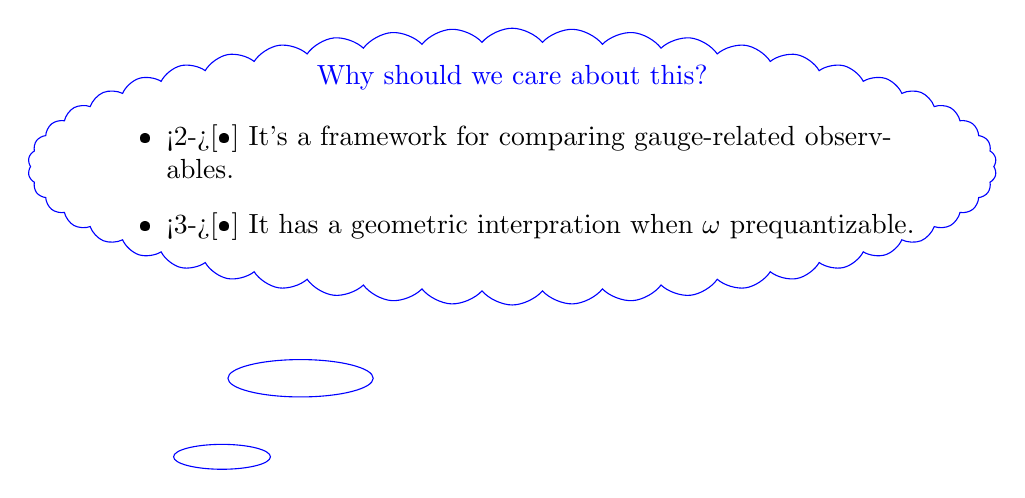
\begin{tikzpicture}
		\node [draw,cloud callout,cloud puffs=50,cloud puff arc=100,blue, minimum height=10em,minimum width=35em,callout relative pointer={(-2,-2)}] (L1) {};
		\node [text width=30em,text centered] (L2) {
			\textcolor{blue}{Why should we care about this?}
			\\
			\begin{itemize}
				\item<2->[•] It's a framework for comparing gauge-related observables.
				\item<3->[•] It has a geometric interpration when $\omega$ \alert{prequantizable}.
			\end{itemize}
			\medskip
		};
	\end{tikzpicture}
	\end{minipage}	
\end{frame}
%-------------------------------------------------------------------------------------------------------------------------------------------------

%-------------------------------------------------------------------------------------------------------------------------------------------------
\begin{frame}[t]{Scope of the talk}
		\begin{center}
		\tcbox[enhanced,frame hidden,borderline={0.5pt}{0pt}{red,dashed}]{	
			\alert{
			\faQuestionCircle \qquad
				{\bf  What happens in the (higher) $n$-plectic case?}
			\qquad \faQuestionCircle		
			}
		}
		\end{center}
		\vfill

	\only<2->{
		{
			\color{UniGreen}
			\par\noindent\rule{\textwidth}{0.4pt}	
			\\ {\bf  Outline of the talk:} \\[-.5em]
			\par\noindent\rule{\textwidth}{0.4pt}			
		}
		\vspace{-1.5em}
		\tableofcontents
	}
\end{frame}
%-------------------------------------------------------------------------------------------------------------------------------------------------







%-------------------------------------------------------------------------------------------------------------------------------------------------
\section{What is \textbf{multisymplectic geometry}?}
\checkpoint	
%-------------------------------------------------------------------------------------------------------------------------------------------------


\begin{frame}[t, fragile]{Multisymplectic manifolds} %Fragile -->workaround tikzcd
	\begin{center}
		$-$ \emph{multisymplectic means \textbf{going higher} in the degree of $\omega$} $-$
	\end{center}
	\pause
	\begin{defblock}[$n$-plectic manifold ~\emph{(Cantrijn, Ibort, De Le\'on)}]
		\includestandalone[width=0.95\textwidth]{Pictures/hyb-Figure_multisym}	
	\end{defblock}
	%
	\vfill
	%
	%
	\pause
	\begin{block}{Examples:}
		\begin{itemize}
			\item[$\bullet$] 1-plectic $=$ symplectic
			\item[$\bullet$] Any oriented $(n+1)$-dimensional manifold is $n$-plectic w.r.t. the volume form.
			\item[$\bullet$] The multicotangent bundle $\Lambda^n T^\ast Q$ is naturally $n$-plectic.
		\end{itemize}
	\end{block}			 
%
	\pause
	\begin{block}{Historical motivation}
		Mechanics: geometrical foundations of \textit{(first-order)} field theories.
		\begin{itemize}
		 \item[•] Kijowski, W. Tulczyjew $(\sim 1979 )$;
		 \item[•] Cariñena, Crampin, Ibort $(\sim 1991 )$;
		 \item[•] Gotay, Isenberg, Marsden, Montgomery $(\sim 1998 )$;
		 \\ $\cdots$
		\end{itemize}
	\end{block}
\end{frame}


%-------------------------------------------------------------------------------------------------------------------------------------------------
\section{What is the \textbf{higher analogue} of the \textbf{Poisson algebra}?}
\checkpoint	
%-------------------------------------------------------------------------------------------------------------------------------------------------


\begin{frame}{Hamiltonian forms}
	\only<1>{
	\medskip
	\begin{columns}[T]
		\setlength{\belowdisplayskip}{5pt}
		\begin{column}{.50\linewidth}
			\centering \it
			$-$ symplectic case $-$
			\vspace{20em}		
		\end{column}	
		%
		\onslide{\vrule{}}
		%
		\begin{column}{.50\linewidth}
			\centering \it
			$-$ $n$-plectic case $-$
			\vspace{20em}		
		\end{column}	
	\end{columns}
	}
	\pause
	%
	\begin{defblock}[Hamiltonian $(n-1)$-forms]
		\begin{displaymath}
			\Omega^{n-1}_{ham}(M,\omega) 	:=
			\biggr\{ \sigma \in  \Omega^{n-1}(M) \; \biggr\vert \; 
				\exists \vHam_\sigma \in \mathfrak{X}(M) ~:~ 
				\tikz[baseline,remember picture]{\node[rounded corners,
                        fill=orange!5,draw=orange!30,anchor=base]            
            			(target) {$d \sigma = -\iota_{\vHam_\sigma} \omega$ };
            	}				
				~\biggr\} 
			\end{displaymath}
	\end{defblock}
	%
	\onslide<2>{
		\tikz[overlay,remember picture]
		{
			\node[rounded corners,
                 fill=orange!5,draw=orange!30,anchor=base]
            	 (base) at ($(current page.north east)-(2,1)$) [rotate=-0,text width=3.5cm,align=center] {\footnotesize{\textcolor{red}{Hamilton-DeDonder-Weyl \\equation}}};
		}	
		\begin{tikzpicture}[overlay,remember picture]
		    	\path[->] (base.south east) edge[bend left,red](target.east);
	    \end{tikzpicture}
	}
	%
	\vspace{-1em}
	\begin{columns}[T]
		\setlength{\belowdisplayskip}{5pt}
		\begin{column}{.50\linewidth}
			%
			\centering \it
			$-$ symplectic case $-$
			\onslide<3->{
			\begin{thmblock}[Observables Poisson algebra]
				$C^\infty(M,\omega)$ endowed with
				\vspace{-.5em}
				\begin{displaymath}
					\lbrace \sigma_1, \sigma_2 \rbrace =			
					~ - \iota_{\vHam_1}\iota_{\vHam_2} \omega 
					~= \mathcal{L}_{\vHam_1} \sigma_2
				\end{displaymath}			
				forms a Poisson algebra.
			\end{thmblock}
			}
			%
			\onslide<4->{
			\vspace{1em}
			\begin{itemize}
				\item[\cmark] Skew-symmetric;
				\item[\cmark] multiplication of observables;
				\item[\cmark] Leibniz Rule;
				\item[\cmark] Jacobi equation;
			\end{itemize}		
			}		
		\end{column}	
		%
		\onslide<1->{\vrule{}}
		%
		\begin{column}{.50\linewidth}
			\centering \it
			$-$ $n$-plectic case $-$
			\onslide<5->{			
			\begin{thmblock}[Observables $L_\infty$-algebra]
				$\Omega^{n-1}_{ham}(M,\omega)$ endowed with
				\vspace{-.5em}
				\begin{displaymath}
					\lbrace \sigma_1, \sigma_2 \rbrace =			
					~ - \iota_{\vHam_1}\iota_{\vHam_2} \omega 
				\end{displaymath}			
				can be "completed" to a \\ $L_\infty-algebra$.
			\end{thmblock}
			}
			%
			\onslide<6->{
			\begin{itemize}
				\item[\cmark] Skew-symmetric;
				\item[\xmark] multiplication of observables;
				\item[\xmark] Jacobi equation;
				%\\ \hspace*{4.25em} full-fledged Jacobi equation;
				\item[\smark] Jacobi equation \emph{up to homotopies}.
			\end{itemize}			
			}
		\end{column}	
	\end{columns}
\end{frame}
%-------------------------------------------------------------------------------------------------------------------------------------------------

%-------------------------------------------------------------------------------------------------------------------------------------------------
\begin{frame}[fragile]{Lie $\infty$-algebra of Observables (higher observables) }
	Let be $(M,\omega)$ a $n$-plectic manifold.
	  	\vfill
	\begin{defblock}[$L_\infty$-algebra of observables ~\emph{(Rogers)}]
		\medskip
		\hspace{.25em} Is a cochain-complex $(L,\{\cdot\}_1)$ \\
		\vspace{-1em}
		\begin{center}
			\includestandalone{Pictures/hyb-Frame_Observables}
		\end{center}
		\onslide<2->{
			\bigskip
			\hspace{.25em} with $n$ (skew-symmetric) multibrackets $(2 \leq k \leq n+1)$\\
			\vspace{-1em}
			\onslide<3->{
				\begin{center}
					\includestandalone{Pictures/Equation_Multibracket}	
				\end{center}
			}
			\medskip
		}
		%
	\end{defblock}
%	\onslide<3->{
%		\emph{Higher analogue} of the \emph{Poisson algebra structure} associated to a symplectic mfd.
%	\vfill
%	\begin{columns}
%		\hfill
%		\begin{column}{.11\linewidth}	
%			If $n>1$:
%			
%		\end{column}	
%		\begin{column}{.8\linewidth}
%		\begin{itemize}
%			\item[\xmark] \textcolor{red}{we lose} :\quad multiplication of observables, Jacobi equation;
%			%\\ \hspace*{4.25em} full-fledged Jacobi equation;
%			\item[\cmark] \textcolor{green}{we gain} :\quad brackets with arities different than two,\\
%			\hspace*{4.25em}
%			 Jacobi equation \emph{up to homotopies}.
%		\end{itemize}		
%		\end{column}		
%	\end{columns}
%	}
  \end{frame}
%-------------------------------------------------------------------------------------------------------------------------------------------------


%-------------------------------------------------------------------------------------------------------------------------------------------------
\section{What is the \textbf{higher analogue} of the \textbf{twisted Lie algebroid}?}
\checkpoint	
%-------------------------------------------------------------------------------------------------------------------------------------------------
%	%- HandOut Flag -----------------------------------------------------------------------------------------
\makeatletter
\@ifundefined{ifHandout}{%
  \expandafter\newif\csname ifHandout\endcsname
}{}
\makeatother

%- D0cum3nt ----------------------------------------------------------------------------------------------
\documentclass[beamer,10pt]{standalone}   
%\documentclass[beamer,10pt,handout]{standalone}  \Handouttrue  

\ifHandout
	\setbeameroption{show notes} %print notes   
\fi

	
%- Packages ----------------------------------------------------------------------------------------------
\usepackage{custom-style}
\usetikzlibrary{positioning}
\usepackage{multicol}


%--Beamer Style-----------------------------------------------------------------------------------------------
\usetheme{toninus}
\usepackage{animate}
\usetikzlibrary{positioning, arrows}
\usetikzlibrary{shapes}

\begin{document}
%-------------------------------------------------------------------------------------------------------------------------------------------------


%-------------------------------------------------------------------------------------------------------------------------------------------------
\subsection{Poisson algebra and Lie algebroids}
%-------------------------------------------------------------------------------------------------------------------------------------------------
%-------------------------------------------------------------------------------------------------------------------------------------------------
\begin{frame}[fragile]{Embedding of the observables algebra in the Lie algebroid}
	Given a \alert{symplectic mfd.} $(M,\omega)$ ...
	\vfill
	\begin{center}
		\includestandalone[width=.95\textwidth]{Pictures/Frame_Embedding_Diagram_symplectic}
	\end{center}
	\vfill
	\begin{minipage}[t][8.5em][t]{\textwidth}
		\begin{itemize}
			\only<1-3>{
			\item<1-> \alert<1>{... there is a naturally associated Poisson algebra ...}
			\item<2-> \alert<2>{... and also a (standard twisted) Lie Algebroid}.
			\item<3-> A Lie algebroid is a "controlled" $\infty$-dimensional Lie algebra given (in this case) by
			\begin{displaymath}
					\left[\binom{x_1}{f_1},\binom{x_2}{f_2}\right]
					~=~
					\binom{[x_1,x_2]}{x_1(f_2)-x_2(f_1)-\omega(x_1,x_2)}
				\end{displaymath}
			}
			\item[]<4->
				\quad\\
				\begin{thmblock}[There exists an embedding of Lie algebras.]
					\begin{displaymath}
						\begin{tikzcd}
							\Psi~:&[-1em] C^{\infty}(M)_\omega \ar[r,"\Psi"]& \Gamma(TM\oplus \mathbb{R})_\omega
							\\[-2em]
							& f \ar[r,mapsto] & \binom{\mathscr{v}_f}{f}
						\end{tikzcd}		
					\end{displaymath}
				\end{thmblock}
		\end{itemize}
	\end{minipage}
\end{frame}
\note{}
%-------------------------------------------------------------------------------------------------------------------------------------------------


%-------------------------------------------------------------------------------------------------------------------------------------------------
\subsection{Compatibility between gauge transformations}
%-------------------------------------------------------------------------------------------------------------------------------------------------
%-------------------------------------------------------------------------------------------------------------------------------------------------
\begin{frame}[fragile]{Compatibility between gauge transformations and comoment maps}
	%
	Consider $(M,\omega)$ \alert{symplectic mfd.}
	%
	\begin{center}
			\includestandalone[width=.8\textwidth]{Pictures/Frame_BigDiagram_symplectic}
	\end{center}
	%
	\vspace{-1em}
	\vfill
	\begin{minipage}[t][8em][t]{\textwidth}
		\begin{itemize}
			\only<2>{
				\item<2-> Consider a second gauge-related symplectic structure on $M$
					\begin{displaymath}
						\tilde{\omega} = \omega + d B \qquad \text{with} \quad B\in \Omega^1(M).
					\end{displaymath}
			}
			\only<3-4>{
				\item<3-> There is a natural isomorphism in the Lie Alg.oids category \emph{($B$-transformation)}
					\begin{displaymath}
						\binom{x}{f} \mapsto \binom{x}{f-\iota_x B} ~.
					\end{displaymath}
			}
			\only<6-7>{
				\item<6-> Consider an infinitesimal group action $\mathfrak{g}\circlearrowleft M$ which is Hamiltonian w.r.t. both $\omega$ and $\tilde{\omega}$.
				\item<7-> let be $f:\mathfrak{g} \to C^\infty(M)_\omega$ and $\tilde{f}:\mathfrak{g} \to C^\infty(M)_{\tilde{\omega}}$ two comoment map s.t.
				\begin{displaymath}
					\tilde{f}(\xi) = f(\xi) - \iota_{\underline{\xi}}B
				\end{displaymath}
				}
			\item[]						
		\end{itemize}
	\only<5>{
		\vspace{-.75em}
		\begin{center}
		\tcbox[enhanced,frame hidden,borderline={0.5pt}{0pt}{red,dashed}]{	
			\alert{
			\faQuestionCircle \qquad
				{How can we close the left-hand side?}
			\qquad \faQuestionCircle		
			}
		}
		\end{center}
	}
	\only<8->{
		\vspace{-.75em}
		\tcbset{colback=white,
		colbacktitle=white,
		colframe=red!70!black,
		boxrule=1pt,
		colupper=red!70!black,
		arc=15pt,
		}
		\begin{tcolorbox}[enhanced,frame hidden,borderline={0.5pt}{0pt}{blue}]
			\color{blue}{
			Lemma: The central pentagon commutes!
			}
		\end{tcolorbox}
	\vfill
	}
	\only<9->{
		\vspace{-.75em}
		\begin{center}
		\tcbox[enhanced,frame hidden,borderline={0.5pt}{0pt}{red,dashed}]{	
			\alert{
			\faQuestionCircle \qquad
				{What happens in the higher (n-plectic) case?}
			\qquad \faQuestionCircle		
			}
		}
		\end{center}
	}
	\end{minipage}	
\end{frame}
\note[itemize]{
	\item The horizontal embedding is  $f \mapsto (v_f,f)$;
	\item Vertical maps are also known as \emph{Gauge transformations}
	\item upshot: 
	\begin{enumerate}
		\item 
	\end{enumerate}
}
%-------------------------------------------------------------------------------------------------------------------------------------------------



%-------------------------------------------------------------------------------------------------------------------------------------------------
\subsection{Geometric interpretation in pre-quantization}
%-------------------------------------------------------------------------------------------------------------------------------------------------
%-------------------------------------------------------------------------------------------------------------------------------------------------
\begin{frame}[fragile]{Geometric interpretation of the diagram}
	%
	Consider $(M,\omega)$ \alert{symplectic} and \alert{\underline{prequantizable}}.
	%
	\begin{center}
			\includestandalone[width=.8\textwidth]{Pictures/Frame_BigDiagram_prequantum}
	\end{center}
	%
	\vspace{-2em}
	\begin{minipage}[t][1.7cm][t]{\textwidth}
	\begin{itemize}
		\only<1-3>{
			\item<1-> Fix a Prequantization Bundle $S^1\hookrightarrow P \to M$ with connection $\theta$,
			\item<2-> "infinitesimal quantomorphisms" $Q(P,\theta):=\lbrace Y \in \mathfrak{X}(P)~|~ \mathcal{L}_Y \theta =0 \}$.
		}
		\item<4-> Embdedding through Atiah algebroid.
	\end{itemize}
	\end{minipage}
	\vfill
	\tcbset{colback=white,
	colbacktitle=white,
	colframe=red!70!black,
	boxrule=1pt,
	colupper=red!70!black,
	arc=15pt,
	}
	\begin{minipage}[t][1.7cm][t]{\textwidth}
	\only<3>{ 
		\begin{tcolorbox}[enhanced,frame hidden,borderline={0.5pt}{0pt}{blue}]
			\color{blue}{
			Lemma: The left square commutes!
			}
		\end{tcolorbox}
	}
	\only<5>{
		\begin{tcolorbox}[enhanced,frame hidden,borderline={0.5pt}{0pt}{blue}]
			\color{blue}{
			Lemma: The left square and right triangle commute!
			}
		\end{tcolorbox}
	}
	\end{minipage}
	%
\end{frame}
\note[itemize]{
	\item questo fatto puramente algebrico ha un'interessante interpretazione nell'ambito della prequantizzaazione  Relevance to Prequantization
	\item The horizontal embedding is  $f \mapsto (v_f,f)$;
	\item Vertical maps are also known as \emph{Gauge transformations}
	\item upshot: 
	\begin{enumerate}
		\item 
	\end{enumerate}
}
%-------------------------------------------------------------------------------------------------------------------------------------------------


\end{document}


%-------------------------------------------------------------------------------------------------------------------------------------------------




\end{document}


%-------------------------------------------------------------------------------------------------------------------------------------------------
\section{What is the \textbf{higher analogue} of the \textbf{comoment map}?}
\checkpoint	
%-------------------------------------------------------------------------------------------------------------------------------------------------
%	%- HandOut Flag -----------------------------------------------------------------------------------------
\makeatletter
\@ifundefined{ifHandout}{%
  \expandafter\newif\csname ifHandout\endcsname
}{}
\makeatother

%- D0cum3nt ----------------------------------------------------------------------------------------------
\documentclass[beamer,10pt]{standalone}   
%\documentclass[beamer,10pt,handout]{standalone}  \Handouttrue  

\ifHandout
	\setbeameroption{show notes} %print notes   
\fi

	
%- Packages ----------------------------------------------------------------------------------------------
\usepackage{custom-style}
\usetikzlibrary{positioning}
\usepackage{multicol}


%--Beamer Style-----------------------------------------------------------------------------------------------
\usetheme{toninus}
\usepackage{animate}
\usetikzlibrary{positioning, arrows}
\usetikzlibrary{shapes}

\begin{document}
%-------------------------------------------------------------------------------------------------------------------------------------------------


%-------------------------------------------------------------------------------------------------------------------------------------------------
\subsection{Poisson algebra and Lie algebroids}
%-------------------------------------------------------------------------------------------------------------------------------------------------
%-------------------------------------------------------------------------------------------------------------------------------------------------
\begin{frame}[fragile]{Embedding of the observables algebra in the Lie algebroid}
	Given a \alert{symplectic mfd.} $(M,\omega)$ ...
	\vfill
	\begin{center}
		\includestandalone[width=.95\textwidth]{Pictures/Frame_Embedding_Diagram_symplectic}
	\end{center}
	\vfill
	\begin{minipage}[t][8.5em][t]{\textwidth}
		\begin{itemize}
			\only<1-3>{
			\item<1-> \alert<1>{... there is a naturally associated Poisson algebra ...}
			\item<2-> \alert<2>{... and also a (standard twisted) Lie Algebroid}.
			\item<3-> A Lie algebroid is a "controlled" $\infty$-dimensional Lie algebra given (in this case) by
			\begin{displaymath}
					\left[\binom{x_1}{f_1},\binom{x_2}{f_2}\right]
					~=~
					\binom{[x_1,x_2]}{x_1(f_2)-x_2(f_1)-\omega(x_1,x_2)}
				\end{displaymath}
			}
			\item[]<4->
				\quad\\
				\begin{thmblock}[There exists an embedding of Lie algebras.]
					\begin{displaymath}
						\begin{tikzcd}
							\Psi~:&[-1em] C^{\infty}(M)_\omega \ar[r,"\Psi"]& \Gamma(TM\oplus \mathbb{R})_\omega
							\\[-2em]
							& f \ar[r,mapsto] & \binom{\mathscr{v}_f}{f}
						\end{tikzcd}		
					\end{displaymath}
				\end{thmblock}
		\end{itemize}
	\end{minipage}
\end{frame}
\note{}
%-------------------------------------------------------------------------------------------------------------------------------------------------


%-------------------------------------------------------------------------------------------------------------------------------------------------
\subsection{Compatibility between gauge transformations}
%-------------------------------------------------------------------------------------------------------------------------------------------------
%-------------------------------------------------------------------------------------------------------------------------------------------------
\begin{frame}[fragile]{Compatibility between gauge transformations and comoment maps}
	%
	Consider $(M,\omega)$ \alert{symplectic mfd.}
	%
	\begin{center}
			\includestandalone[width=.8\textwidth]{Pictures/Frame_BigDiagram_symplectic}
	\end{center}
	%
	\vspace{-1em}
	\vfill
	\begin{minipage}[t][8em][t]{\textwidth}
		\begin{itemize}
			\only<2>{
				\item<2-> Consider a second gauge-related symplectic structure on $M$
					\begin{displaymath}
						\tilde{\omega} = \omega + d B \qquad \text{with} \quad B\in \Omega^1(M).
					\end{displaymath}
			}
			\only<3-4>{
				\item<3-> There is a natural isomorphism in the Lie Alg.oids category \emph{($B$-transformation)}
					\begin{displaymath}
						\binom{x}{f} \mapsto \binom{x}{f-\iota_x B} ~.
					\end{displaymath}
			}
			\only<6-7>{
				\item<6-> Consider an infinitesimal group action $\mathfrak{g}\circlearrowleft M$ which is Hamiltonian w.r.t. both $\omega$ and $\tilde{\omega}$.
				\item<7-> let be $f:\mathfrak{g} \to C^\infty(M)_\omega$ and $\tilde{f}:\mathfrak{g} \to C^\infty(M)_{\tilde{\omega}}$ two comoment map s.t.
				\begin{displaymath}
					\tilde{f}(\xi) = f(\xi) - \iota_{\underline{\xi}}B
				\end{displaymath}
				}
			\item[]						
		\end{itemize}
	\only<5>{
		\vspace{-.75em}
		\begin{center}
		\tcbox[enhanced,frame hidden,borderline={0.5pt}{0pt}{red,dashed}]{	
			\alert{
			\faQuestionCircle \qquad
				{How can we close the left-hand side?}
			\qquad \faQuestionCircle		
			}
		}
		\end{center}
	}
	\only<8->{
		\vspace{-.75em}
		\tcbset{colback=white,
		colbacktitle=white,
		colframe=red!70!black,
		boxrule=1pt,
		colupper=red!70!black,
		arc=15pt,
		}
		\begin{tcolorbox}[enhanced,frame hidden,borderline={0.5pt}{0pt}{blue}]
			\color{blue}{
			Lemma: The central pentagon commutes!
			}
		\end{tcolorbox}
	\vfill
	}
	\only<9->{
		\vspace{-.75em}
		\begin{center}
		\tcbox[enhanced,frame hidden,borderline={0.5pt}{0pt}{red,dashed}]{	
			\alert{
			\faQuestionCircle \qquad
				{What happens in the higher (n-plectic) case?}
			\qquad \faQuestionCircle		
			}
		}
		\end{center}
	}
	\end{minipage}	
\end{frame}
\note[itemize]{
	\item The horizontal embedding is  $f \mapsto (v_f,f)$;
	\item Vertical maps are also known as \emph{Gauge transformations}
	\item upshot: 
	\begin{enumerate}
		\item 
	\end{enumerate}
}
%-------------------------------------------------------------------------------------------------------------------------------------------------



%-------------------------------------------------------------------------------------------------------------------------------------------------
\subsection{Geometric interpretation in pre-quantization}
%-------------------------------------------------------------------------------------------------------------------------------------------------
%-------------------------------------------------------------------------------------------------------------------------------------------------
\begin{frame}[fragile]{Geometric interpretation of the diagram}
	%
	Consider $(M,\omega)$ \alert{symplectic} and \alert{\underline{prequantizable}}.
	%
	\begin{center}
			\includestandalone[width=.8\textwidth]{Pictures/Frame_BigDiagram_prequantum}
	\end{center}
	%
	\vspace{-2em}
	\begin{minipage}[t][1.7cm][t]{\textwidth}
	\begin{itemize}
		\only<1-3>{
			\item<1-> Fix a Prequantization Bundle $S^1\hookrightarrow P \to M$ with connection $\theta$,
			\item<2-> "infinitesimal quantomorphisms" $Q(P,\theta):=\lbrace Y \in \mathfrak{X}(P)~|~ \mathcal{L}_Y \theta =0 \}$.
		}
		\item<4-> Embdedding through Atiah algebroid.
	\end{itemize}
	\end{minipage}
	\vfill
	\tcbset{colback=white,
	colbacktitle=white,
	colframe=red!70!black,
	boxrule=1pt,
	colupper=red!70!black,
	arc=15pt,
	}
	\begin{minipage}[t][1.7cm][t]{\textwidth}
	\only<3>{ 
		\begin{tcolorbox}[enhanced,frame hidden,borderline={0.5pt}{0pt}{blue}]
			\color{blue}{
			Lemma: The left square commutes!
			}
		\end{tcolorbox}
	}
	\only<5>{
		\begin{tcolorbox}[enhanced,frame hidden,borderline={0.5pt}{0pt}{blue}]
			\color{blue}{
			Lemma: The left square and right triangle commute!
			}
		\end{tcolorbox}
	}
	\end{minipage}
	%
\end{frame}
\note[itemize]{
	\item questo fatto puramente algebrico ha un'interessante interpretazione nell'ambito della prequantizzaazione  Relevance to Prequantization
	\item The horizontal embedding is  $f \mapsto (v_f,f)$;
	\item Vertical maps are also known as \emph{Gauge transformations}
	\item upshot: 
	\begin{enumerate}
		\item 
	\end{enumerate}
}
%-------------------------------------------------------------------------------------------------------------------------------------------------


\end{document}


%-------------------------------------------------------------------------------------------------------------------------------------------------




\end{document}



%-------------------------------------------------------------------------------------------------------------------------------------------------
\section{Does the \textbf{higher pentagonal diagram commute}?}
\checkpoint	
%-------------------------------------------------------------------------------------------------------------------------------------------------
%	%- HandOut Flag -----------------------------------------------------------------------------------------
\makeatletter
\@ifundefined{ifHandout}{%
  \expandafter\newif\csname ifHandout\endcsname
}{}
\makeatother

%- D0cum3nt ----------------------------------------------------------------------------------------------
\documentclass[beamer,10pt]{standalone}   
%\documentclass[beamer,10pt,handout]{standalone}  \Handouttrue  

\ifHandout
	\setbeameroption{show notes} %print notes   
\fi

	
%- Packages ----------------------------------------------------------------------------------------------
\usepackage{custom-style}
\usetikzlibrary{positioning}
\usepackage{multicol}


%--Beamer Style-----------------------------------------------------------------------------------------------
\usetheme{toninus}
\usepackage{animate}
\usetikzlibrary{positioning, arrows}
\usetikzlibrary{shapes}

\begin{document}
%-------------------------------------------------------------------------------------------------------------------------------------------------


%-------------------------------------------------------------------------------------------------------------------------------------------------
\subsection{Poisson algebra and Lie algebroids}
%-------------------------------------------------------------------------------------------------------------------------------------------------
%-------------------------------------------------------------------------------------------------------------------------------------------------
\begin{frame}[fragile]{Embedding of the observables algebra in the Lie algebroid}
	Given a \alert{symplectic mfd.} $(M,\omega)$ ...
	\vfill
	\begin{center}
		\includestandalone[width=.95\textwidth]{Pictures/Frame_Embedding_Diagram_symplectic}
	\end{center}
	\vfill
	\begin{minipage}[t][8.5em][t]{\textwidth}
		\begin{itemize}
			\only<1-3>{
			\item<1-> \alert<1>{... there is a naturally associated Poisson algebra ...}
			\item<2-> \alert<2>{... and also a (standard twisted) Lie Algebroid}.
			\item<3-> A Lie algebroid is a "controlled" $\infty$-dimensional Lie algebra given (in this case) by
			\begin{displaymath}
					\left[\binom{x_1}{f_1},\binom{x_2}{f_2}\right]
					~=~
					\binom{[x_1,x_2]}{x_1(f_2)-x_2(f_1)-\omega(x_1,x_2)}
				\end{displaymath}
			}
			\item[]<4->
				\quad\\
				\begin{thmblock}[There exists an embedding of Lie algebras.]
					\begin{displaymath}
						\begin{tikzcd}
							\Psi~:&[-1em] C^{\infty}(M)_\omega \ar[r,"\Psi"]& \Gamma(TM\oplus \mathbb{R})_\omega
							\\[-2em]
							& f \ar[r,mapsto] & \binom{\mathscr{v}_f}{f}
						\end{tikzcd}		
					\end{displaymath}
				\end{thmblock}
		\end{itemize}
	\end{minipage}
\end{frame}
\note{}
%-------------------------------------------------------------------------------------------------------------------------------------------------


%-------------------------------------------------------------------------------------------------------------------------------------------------
\subsection{Compatibility between gauge transformations}
%-------------------------------------------------------------------------------------------------------------------------------------------------
%-------------------------------------------------------------------------------------------------------------------------------------------------
\begin{frame}[fragile]{Compatibility between gauge transformations and comoment maps}
	%
	Consider $(M,\omega)$ \alert{symplectic mfd.}
	%
	\begin{center}
			\includestandalone[width=.8\textwidth]{Pictures/Frame_BigDiagram_symplectic}
	\end{center}
	%
	\vspace{-1em}
	\vfill
	\begin{minipage}[t][8em][t]{\textwidth}
		\begin{itemize}
			\only<2>{
				\item<2-> Consider a second gauge-related symplectic structure on $M$
					\begin{displaymath}
						\tilde{\omega} = \omega + d B \qquad \text{with} \quad B\in \Omega^1(M).
					\end{displaymath}
			}
			\only<3-4>{
				\item<3-> There is a natural isomorphism in the Lie Alg.oids category \emph{($B$-transformation)}
					\begin{displaymath}
						\binom{x}{f} \mapsto \binom{x}{f-\iota_x B} ~.
					\end{displaymath}
			}
			\only<6-7>{
				\item<6-> Consider an infinitesimal group action $\mathfrak{g}\circlearrowleft M$ which is Hamiltonian w.r.t. both $\omega$ and $\tilde{\omega}$.
				\item<7-> let be $f:\mathfrak{g} \to C^\infty(M)_\omega$ and $\tilde{f}:\mathfrak{g} \to C^\infty(M)_{\tilde{\omega}}$ two comoment map s.t.
				\begin{displaymath}
					\tilde{f}(\xi) = f(\xi) - \iota_{\underline{\xi}}B
				\end{displaymath}
				}
			\item[]						
		\end{itemize}
	\only<5>{
		\vspace{-.75em}
		\begin{center}
		\tcbox[enhanced,frame hidden,borderline={0.5pt}{0pt}{red,dashed}]{	
			\alert{
			\faQuestionCircle \qquad
				{How can we close the left-hand side?}
			\qquad \faQuestionCircle		
			}
		}
		\end{center}
	}
	\only<8->{
		\vspace{-.75em}
		\tcbset{colback=white,
		colbacktitle=white,
		colframe=red!70!black,
		boxrule=1pt,
		colupper=red!70!black,
		arc=15pt,
		}
		\begin{tcolorbox}[enhanced,frame hidden,borderline={0.5pt}{0pt}{blue}]
			\color{blue}{
			Lemma: The central pentagon commutes!
			}
		\end{tcolorbox}
	\vfill
	}
	\only<9->{
		\vspace{-.75em}
		\begin{center}
		\tcbox[enhanced,frame hidden,borderline={0.5pt}{0pt}{red,dashed}]{	
			\alert{
			\faQuestionCircle \qquad
				{What happens in the higher (n-plectic) case?}
			\qquad \faQuestionCircle		
			}
		}
		\end{center}
	}
	\end{minipage}	
\end{frame}
\note[itemize]{
	\item The horizontal embedding is  $f \mapsto (v_f,f)$;
	\item Vertical maps are also known as \emph{Gauge transformations}
	\item upshot: 
	\begin{enumerate}
		\item 
	\end{enumerate}
}
%-------------------------------------------------------------------------------------------------------------------------------------------------



%-------------------------------------------------------------------------------------------------------------------------------------------------
\subsection{Geometric interpretation in pre-quantization}
%-------------------------------------------------------------------------------------------------------------------------------------------------
%-------------------------------------------------------------------------------------------------------------------------------------------------
\begin{frame}[fragile]{Geometric interpretation of the diagram}
	%
	Consider $(M,\omega)$ \alert{symplectic} and \alert{\underline{prequantizable}}.
	%
	\begin{center}
			\includestandalone[width=.8\textwidth]{Pictures/Frame_BigDiagram_prequantum}
	\end{center}
	%
	\vspace{-2em}
	\begin{minipage}[t][1.7cm][t]{\textwidth}
	\begin{itemize}
		\only<1-3>{
			\item<1-> Fix a Prequantization Bundle $S^1\hookrightarrow P \to M$ with connection $\theta$,
			\item<2-> "infinitesimal quantomorphisms" $Q(P,\theta):=\lbrace Y \in \mathfrak{X}(P)~|~ \mathcal{L}_Y \theta =0 \}$.
		}
		\item<4-> Embdedding through Atiah algebroid.
	\end{itemize}
	\end{minipage}
	\vfill
	\tcbset{colback=white,
	colbacktitle=white,
	colframe=red!70!black,
	boxrule=1pt,
	colupper=red!70!black,
	arc=15pt,
	}
	\begin{minipage}[t][1.7cm][t]{\textwidth}
	\only<3>{ 
		\begin{tcolorbox}[enhanced,frame hidden,borderline={0.5pt}{0pt}{blue}]
			\color{blue}{
			Lemma: The left square commutes!
			}
		\end{tcolorbox}
	}
	\only<5>{
		\begin{tcolorbox}[enhanced,frame hidden,borderline={0.5pt}{0pt}{blue}]
			\color{blue}{
			Lemma: The left square and right triangle commute!
			}
		\end{tcolorbox}
	}
	\end{minipage}
	%
\end{frame}
\note[itemize]{
	\item questo fatto puramente algebrico ha un'interessante interpretazione nell'ambito della prequantizzaazione  Relevance to Prequantization
	\item The horizontal embedding is  $f \mapsto (v_f,f)$;
	\item Vertical maps are also known as \emph{Gauge transformations}
	\item upshot: 
	\begin{enumerate}
		\item 
	\end{enumerate}
}
%-------------------------------------------------------------------------------------------------------------------------------------------------


\end{document}


%-------------------------------------------------------------------------------------------------------------------------------------------------




\end{document}



%------------------------------------------------------------------------------------------------
% APPENDIX
%------------------------------------------------------------------------------------------------
\appendix
%-------------------------------------------------------------------------------------------------------------------------------------------------
\section{Complementary Material}
%	%+----------------------------------------------------------------------------+
%| SLIDES: 
%| Chapter: Complementary material - details on eventual questions
%| Author: Antonio miti
%| Event: PHD preliminary Defence
%+----------------------------------------------------------------------------+

%- HandOut Flag -----------------------------------------------------------------------------------------
\newif\ifHandout

%- D0cum3nt ----------------------------------------------------------------------------------------------
\documentclass[beamer,10pt]{standalone}   
%\documentclass[beamer,10pt,handout]{standalone}  \Handouttrue  

%- HandOut Flag -----------------------------------------------------------------------------------------
\ifHandout
	\setbeameroption{show notes} %print notes   
\fi

	
%- Packages ----------------------------------------------------------------------------------------------
\usepackage{custom-style}

%--Beamer Style-----------------------------------------------------------------------------------------------
\usetheme{toninus}



\providecommand{\blank}{\text{\textvisiblespace}}


\newcommand{\subsectiontitle}{
  \begin{frame}
  \vfill
  \centering
  \begin{beamercolorbox}[sep=8pt,center,shadow=true,rounded=true]{title}
    \usebeamerfont{title}\insertsectionhead\par%
    \usebeamerfont{title}\insertsubsectionhead\par%
  \end{beamercolorbox}
  \vfill
  \end{frame}
}

\providecommand{\blank}{\text{\textvisiblespace}}




%---------------------------------------------------------------------------------------------------------------------------------------------------
%- D0cum3nt ----------------------------------------------------------------------------------------------------------------------------------
\begin{document}
%------------------------------------------------------------------------------------------------

%##################################################################################
\begin{frame}
	\begin{center}
	\Huge\emph{Supplementary Material}
	\end{center}
\end{frame}
\note[itemize]{
	\item
}
\addtocounter{framenumber}{-1}
%##################################################################################





%===================================================================================
\section{Background}
%===================================================================================



%-------------------------------------------------------------------------------------------------------------------------------------------------
\subsection{MultiSymplectic Geometry}
%-------------------------------------------------------------------------------------------------------------------------------------------------

%-------------------------------------------------------------------------------------------------------------------------------------------------
\begin{frame}[fragile]{Multisymplectic geometry in a nutshell}
	\begin{block}{Historical motivation}
		Mechanics: geometrical foundations of \textit{(first-order)} field theories.
	\end{block}
	\vfill	
	\begin{table}
		\only<2>{
		\begin{tabular}{|p{0.2\textwidth}|p{0.3\textwidth}|p{0.35\textwidth}|} 
            \hline
            \parbox[][20pt][c]{0.2\textwidth}{mechanics} & \multicolumn{2}{c|}{geometry} \\
            \hline
            \parbox[][20pt][c]{0.2\textwidth}{phase space} & symplectic manifold &  \\[.25em]
            \parbox[][20pt][c]{0.2\textwidth}{classical \\ observables} & Poisson algebra &  \\[.25em]
            \parbox[][20pt][c]{0.2\textwidth}{symmetries} &  group actions admitting comoment map &  
            \\
            \hline
  \multicolumn{1}{c}{}
            &  \multicolumn{1}{@{}c@{}}{$\underbrace{\hspace*{.3\textwidth}}_{\text{point-like particles systems}}$} 
            &  \multicolumn{1}{@{}c@{}}{}              \\
		\end{tabular}
		
		
		}
		\onslide<3->{
		\begin{tabular}{|p{0.2\textwidth}|p{0.3\textwidth}|p{0.35\textwidth}|} 
            \hline
            \parbox[][20pt][c]{0.2\textwidth}{mechanics} & \multicolumn{2}{c|}{geometry} \\
            \hline
            \parbox[][20pt][c]{0.2\textwidth}{phase space} & symplectic manifold & multisymplectic manifold \\[.25em]
            \parbox[][20pt][c]{0.2\textwidth}{classical \\ observables} & Poisson algebra & $L_\infty$-algebra \\[.25em]
            \parbox[][20pt][c]{0.2\textwidth}{symmetries} &  group actions admitting comoment map & group actions admitting 
			\tikz[baseline,remember picture]{\node[rounded corners,
                        fill=orange!10,draw=orange!30,anchor=base]            
            			(target) {homotopy comomentum map};
            }
            \\
            \hline
  \multicolumn{1}{c}{}
            &  \multicolumn{1}{@{}c@{}}{$\underbrace{\hspace*{.3\textwidth}}_{\text{point-like particles systems}}$} 
            &
            \multicolumn{1}{@{}c@{}}{$\underbrace{\hspace*{.3\textwidth}}_{\text{field-theoretic systems}}$} 
               \\
		\end{tabular}
		}
	\end{table}		
	\vfill
	\onslide<4->{
	
	\begin{block}{Scope of the thesis}
		\begin{itemize}
			\item[$\bullet$] Develop theory of 
				\tikz[baseline,remember picture]{\node[rounded corners,
                        fill=orange!10,draw=orange!30,anchor=base]            
            			(base) {homotopy comomentum maps};
            	}
            \item[$\bullet$] produce new meaningful examples.
		\end{itemize}
	\end{block}


                    \begin{tikzpicture}[overlay,remember picture]
                    \path[->]<4-> (base.north east) edge[bend right](target.south east);
                    \end{tikzpicture}
	}


\end{frame}
\note[itemize]{
	\item Historically, the interest in multisymplectic manifolds, has been motivated by the need for understanding the geometrical foundations of first-order classical field theories.
	The key point is that, just as one can associate a symplectic manifold to an ordinary classical mechanical system (e.g. a single
point-like particle constrained to some manifold), it is possible to associate a multisymplectic
manifold to any classical field system (e.g. a continuous medium like a filament or a fluid). See frame Extra-\ref{Frame:Ms-Field-Mechanics} 
	
	\item General ideas basic parallelisms with caveats
	\item caveat: points in multiphase spaces are not states
	\item the table hides the duality between geometric and algebraic approaches to the problem.
	\item 
}
%-------------------------------------------------------------------------------------------------------------------------------------------------


%-------------------------------------------------------------------------------------------------------------------------------------------------
\begin{frame}[fragile]{Multisymplectic manifolds} %Fragile -->workaround tikzcd
	\begin{defblock}[$n$-plectic manifold ~\emph{(Cantrijn, Ibort, De Le\'on)}]
	\includestandalone[width=0.95\textwidth]{Pictures/Figure_multisym}	
	\end{defblock}
	%
	\begin{defblock}[Non-degenerate $(n+1)$-form]
		\begin{columns}
			\begin{column}{.45\linewidth}
				\centering{
				The $\omega^\flat$ (flat) bundle map is injective.
				}
			\end{column}
			\begin{column}{.5\linewidth}
						\vspace{-.5em}
				\[
				\begin{tikzcd}[column sep= small,row sep=0ex,
				/tikz/column 1/.append style={anchor=base east}]
				    \omega^\flat \colon T M \ar[r]& \Lambda^n T^\ast M \\
  						 (x,u) \ar[r, mapsto]& (x,\iota_{u} \omega_x)						
				\end{tikzcd}	
				\]
			\end{column}
		\end{columns}
	\end{defblock}
	%
	\pause
	\begin{defblock}[Hamiltonian $(n-1)$-forms]
		\begin{displaymath}
			\Omega^{n-1}_{ham}(M,\omega) 	:=
			\biggr\{ \sigma \in  \Omega^{n-1}(M) \; \biggr\vert \; 
				\exists \mathscr{v}_\sigma \in \mathfrak{X}(M) ~:~ 
				\tikz[baseline,remember picture]{\node[rounded corners,
                        fill=orange!5,draw=orange!30,anchor=base]            
            			(target) {$d \sigma = -\iota_{\mathscr{v}_\sigma} \omega$ };
            	}				
				~\biggr\} 
			\end{displaymath}
	\end{defblock}
	%
	%
	\pause
		\tikz[overlay,remember picture]
		{
			\node[rounded corners,
                 fill=orange!5,draw=orange!30,anchor=base]            
            	 (base) at ($(current page.east)-(2.25,1.8)$) [rotate=-0,text width=4cm,align=center] {\footnotesize{\textcolor{red}{Hamilton-DeDonder-Weyl \\equation}}};
		}	
	\begin{tikzpicture}[overlay,remember picture]
    	\path[->] (base.west) edge[bend left,red](target.south west);
    \end{tikzpicture}	
	\pause
	\vfill
	%
	\begin{block}{Examples:}
		\vspace{-.5em}
		\setbeamercovered{transparent}
		\begin{itemize}[<+->]
			\item[$\bullet$] $n=1$ \qquad\qquad\qquad $\Rightarrow$\quad $\omega$ is a symplectic form
			\item[$\bullet$]  $n=(dim(M)-1)$ \quad$\Rightarrow$\quad $\omega$ is a volume form
			%Any oriented $(n+1)$-dimensional manifold is $n$-plectic w.r.t. the volume form.
			%\item[$\bullet$] Let $G$ a semisimple Lie group and $\langle\cdot,\cdot \rangle$  its killing form. Then $\langle [\cdot,\cdot],\cdot \rangle$ extends to a biinvariant multisymplectic form $\omega$.
			\item[$\bullet$] Let $Q$ a smooth manifold, the multicotangent bundle $\Lambda^n T^\ast Q$ is naturally $n$-plectic.%
			\quad
			\textit{(cfr, \href{https://arxiv.org/abs/physics/9801019}{GIMMSY} construction for classical field theories)}
		\end{itemize}
	\end{block}			 
	
%
\end{frame}
\note[itemize]{
	\item Multisymplectic ($n$-plectic) geometry is a generalization of symplectic geometry where a closed, non degenerate $n+1$-form $(n\geq 1)$  takes the place of the symplectic 2-form
	
	\item multisymplectic means \emph{going higher} in the degree of $\omega$
	
	\item non degeneracy means $\iota_v\omega = 0 \Leftrightarrow v=0$.
	
	\item examples 
		\begin{itemize}
			\item[$\bullet$] 1-plectic $=$ symplectic
			\item[$\bullet$] Any oriented $(n+1)$-dimensional manifold is $n$-plectic w.r.t. the volume form.
			\item[$\bullet$] The multicotangent bundle $\Lambda^n T^\ast Q$ is naturally $n$-plectic.
		\end{itemize}
	
	\item We recognize the special class of forms, called Hamiltonian, determining the Hamiltonian vector fields. 
	Not every $n-1$ form admits an Hamiltonian vector field.
	When it exists, non degeneracy guarantees unicity.
	
	\item Observe also that, by degree reason, when $n$ is equal to $1$ or $dim(M)+1$ an injective flat map $\flat$ is also bijective.
	
	\item It is important to stress that mechanical systems are not the only source instances of this class of of structures. 
				e.g. any semisimple Lie groups has associated a 2-plectic structure and any oriented $n+1$ dimensional manifold is naturally $n$-plectic.
				

}
%---------------------------------------------------------------------------------------------------------------------------------------------------



































\subsection{References}
%------------------------------------------------------------------------------------------------
% https://en.wikibooks.org/wiki/LaTeX/Bibliographies_with_biblatex_and_biber
\begin{frame}[t,allowframebreaks]{Extended Bibliography}
	\bibliographystyle{alpha}
	\bibliography{bibfile}
\end{frame}
%------------------------------------------------------------------------------------------------


%------------------------------------------------------------------------------------------------
\end{document}

%------------------------------------------------------------------------------------------------










%------------------------------------------------------------------------------------------------
\end{document}

